\chapter{Simulated Polynomial Regression } \label{apx:simulated-joint}

\begin{figure}[htbp]
    \centering
    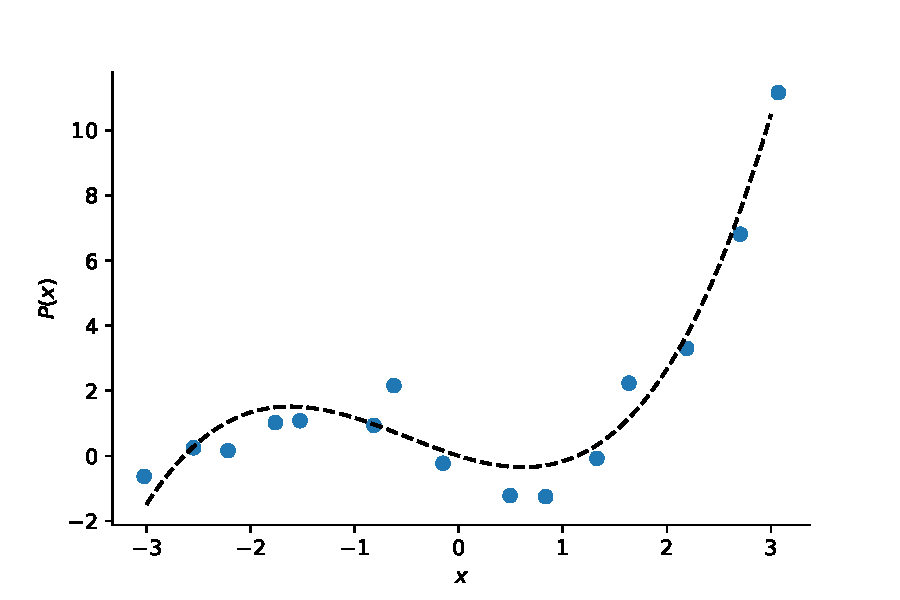
\includegraphics{Figures/pol_model.pdf}
    \caption{Polynomial model and simulated training data.}
    \label{fig:pol-model}
\end{figure}

\begin{figure}[htbp]
    \centering
    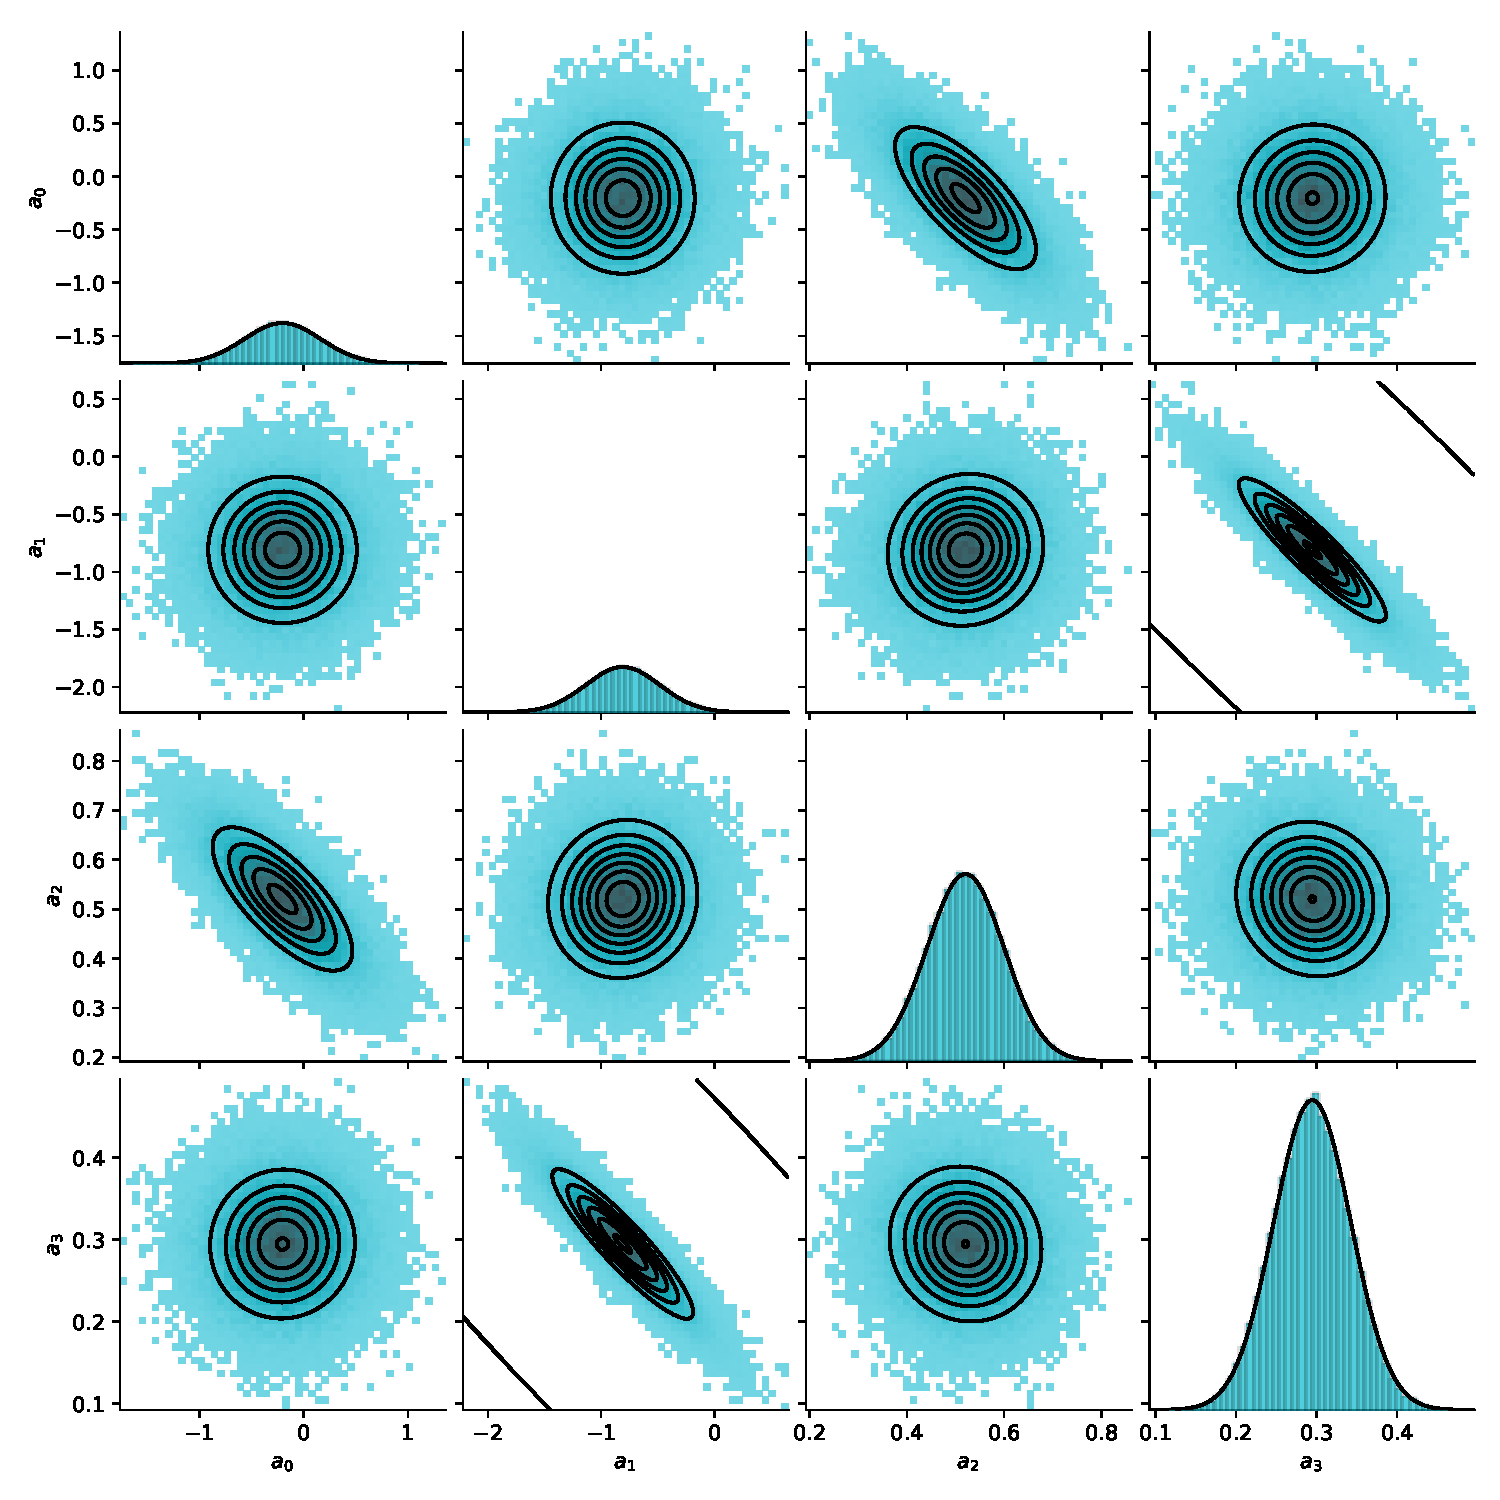
\includegraphics[width=\linewidth]{Figures/simulated_pairs_HMC_15.pdf}
    \caption{Pairwise joint distributions of samples from polynomial Bayesian regressison example, using the HMC algorithm conditioned on every datapoint.}
    \label{fig:pairs-hmc-15}
\end{figure}
\begin{figure}[htbp]
    \centering
    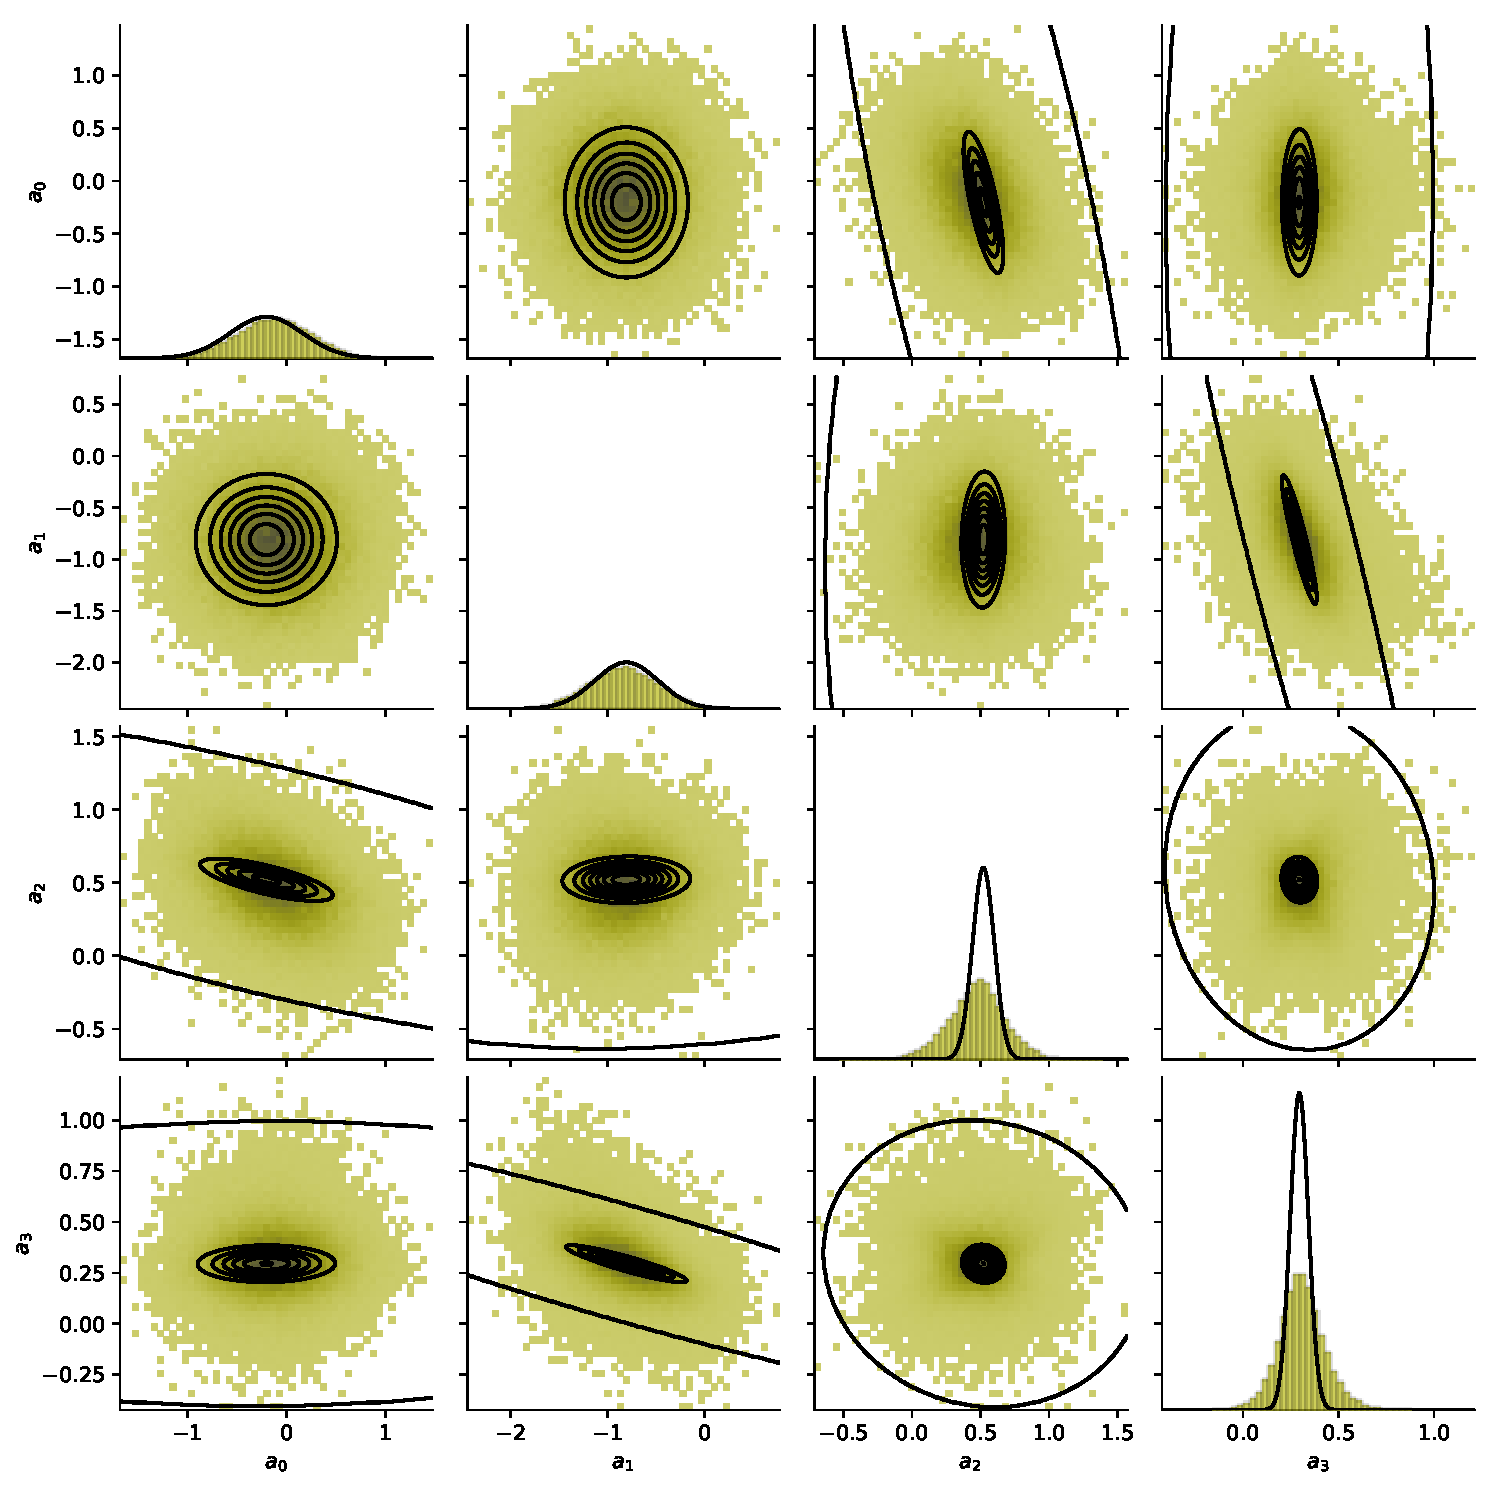
\includegraphics[width=\linewidth]{Figures/simulated_pairs_HMC_5.pdf}
    \caption{Pairwise joint distributions of samples from polynomial Bayesian regressison example, using the naive batched HMC algorithm using a batch size of 5.}
    \label{fig:pairs-hmc-5}
\end{figure}
\begin{figure}[htbp]
    \centering
    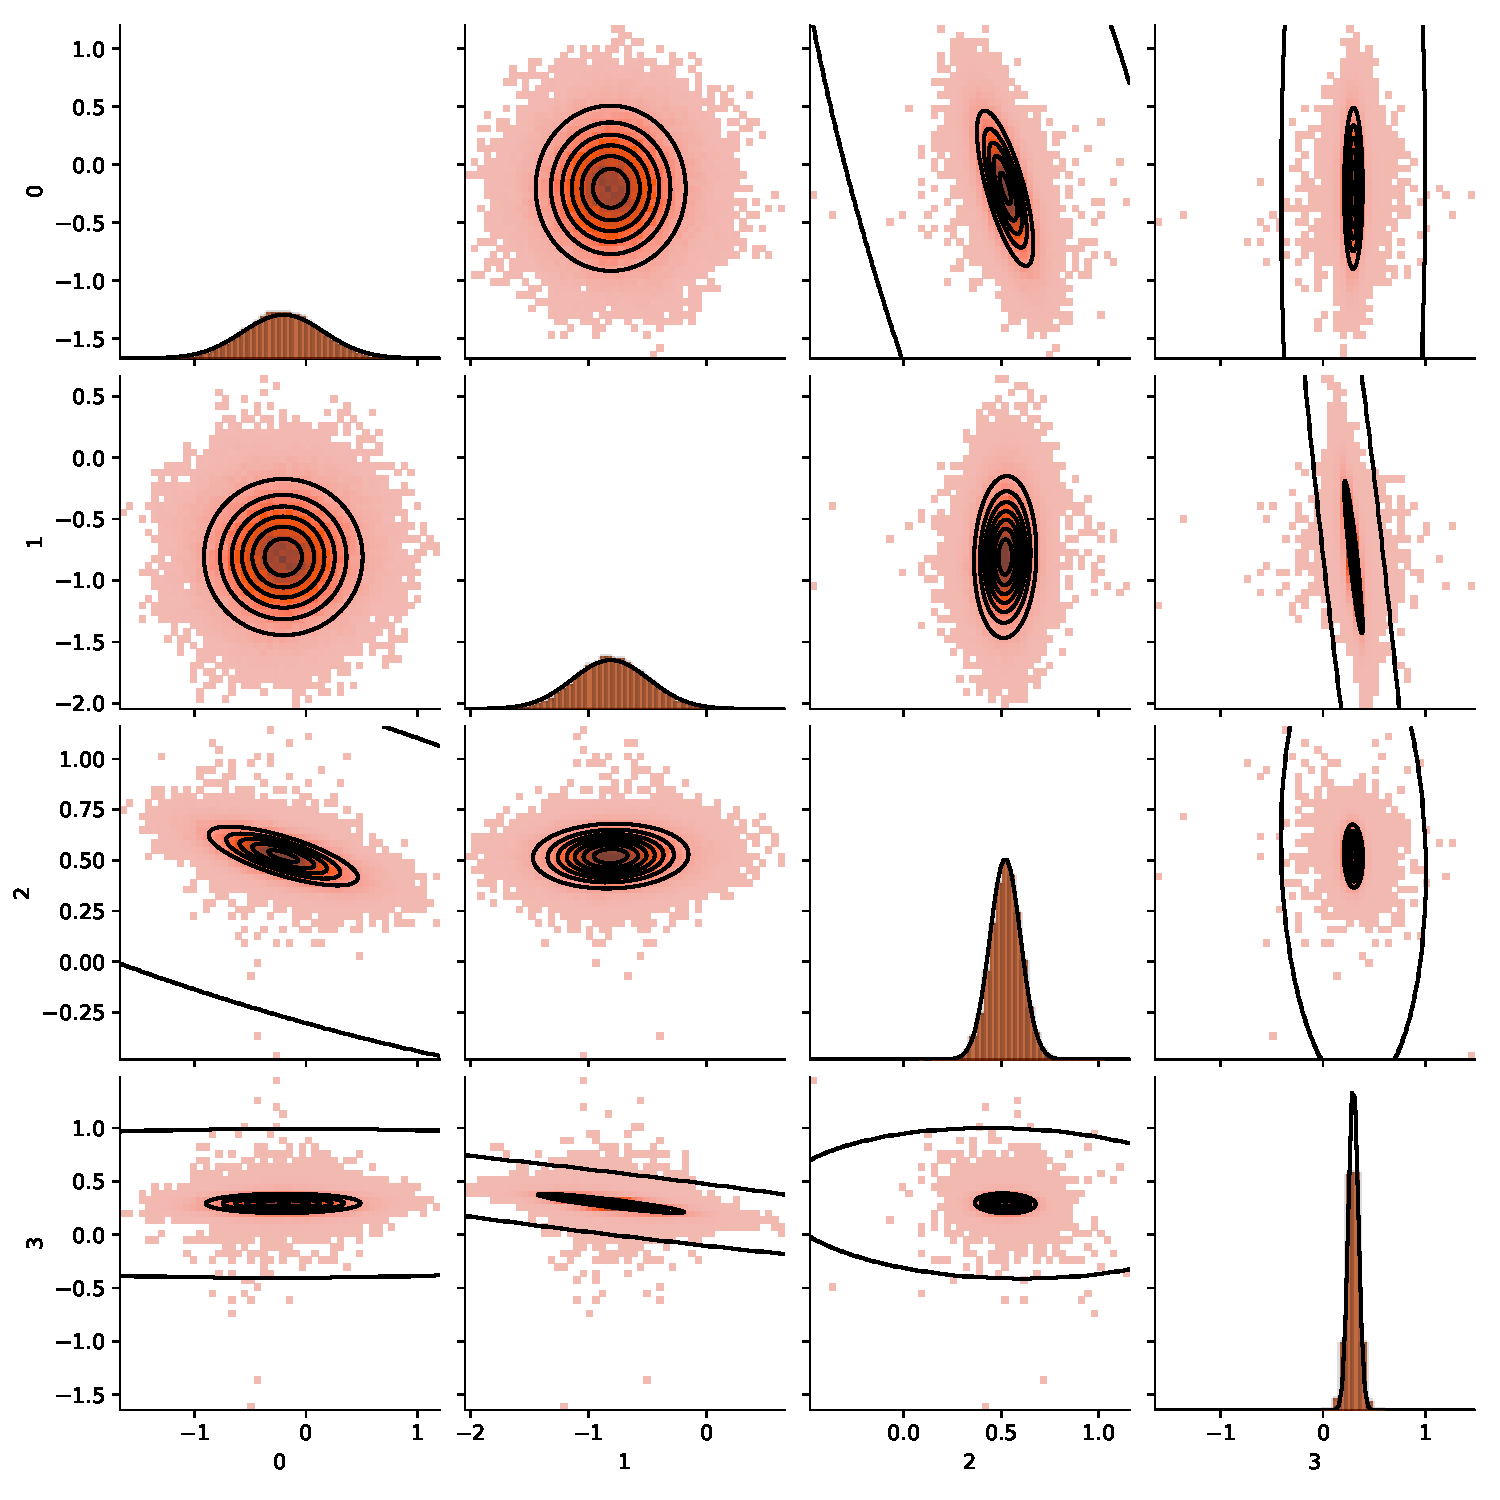
\includegraphics[width=\linewidth]{Figures/simulated_pairs_SGHMC_5.pdf}
    \caption{Pairwise joint distributions of samples from polynomial Bayesian regressison example, using the SGHMC algorithm using a batch size of 5.}
    \label{fig:pairs-sghmc-5}
\end{figure}

\begin{figure}[htbp]
    \centering
    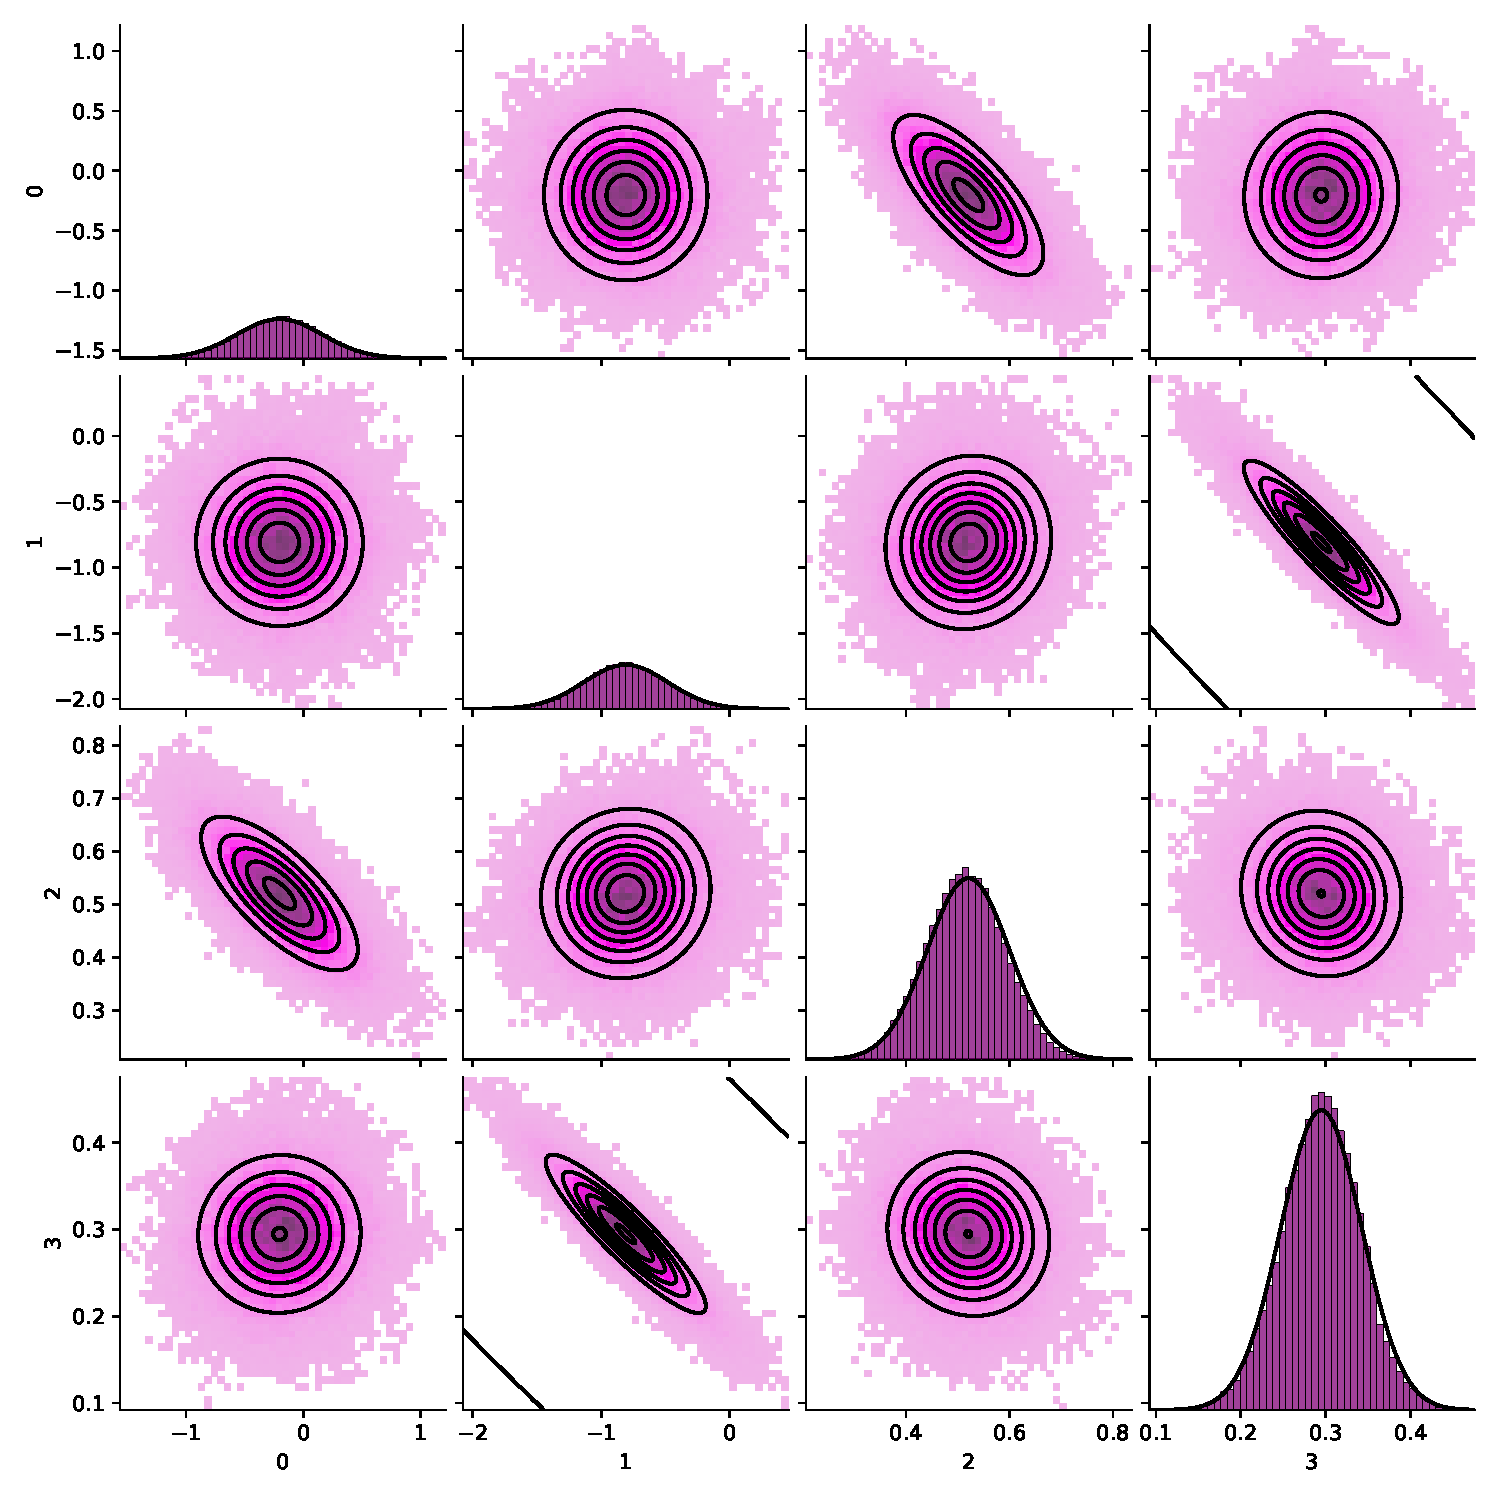
\includegraphics[width=\linewidth]{Figures/simulated_pairs_SGHMCWithVarianceEstimator_5.pdf}
    \caption{Pairwise joint distributions of samples from polynomial Bayesian regressison example, using the SGHMC algorithm with gradient variance estimation  and a batch size of 5.}
    \label{fig:pairs-sghmc-var-est-5}
\end{figure}

\FloatBarrier
\chapter{Hyperparameter Sweeps} 

\section{MNIST} \label{apx:mnist-sweep}



\begin{table}[H]
    \centering
    \resizebox{
        \ifdim\width>\columnwidth
        \columnwidth
      \else
        \width
      \fi
    }{!}{\small
    \begin{tabular}{lp{2.3cm}p{2.3cm}p{2.3cm}p{2.3cm}p{2.3cm}}
\toprule
{} &  Val. error &         \texttt{lr} &  \texttt{log\_sigma\_1} &  \texttt{log\_sigma\_2} &  \texttt{mixture\_ratio} \\
trial &             &                     &                         &                         &                          \\
\midrule
15    &      0.0193 & $3.92\times10^{-4}$ &                       0 &                      -7 &                 0.704007 \\
2     &      0.0202 & $8.71\times10^{-5}$ &                       0 &                      -6 &                 0.643522 \\
5     &      0.0202 & $2.66\times10^{-5}$ &                       0 &                      -8 &                 0.524438 \\
1     &      0.0207 & $7.55\times10^{-5}$ &                       0 &                      -8 &                 0.283183 \\
10    &      0.0207 & $1.32\times10^{-4}$ &                       0 &                      -6 &                 0.562885 \\
11    &      0.0209 & $1.53\times10^{-5}$ &                       0 &                      -8 &                 0.496544 \\
6     &      0.0211 & $6.19\times10^{-4}$ &                      -1 &                      -6 &                 0.640225 \\
12    &      0.0211 & $6.83\times10^{-5}$ &                       0 &                      -8 &                 0.700414 \\
13    &      0.0211 & $3.76\times10^{-5}$ &                       0 &                      -6 &                 0.654232 \\
8     &      0.0213 & $2.59\times10^{-4}$ &                      -1 &                      -6 &                 0.400428 \\
\bottomrule
\end{tabular}

    }
    \caption{Top hyperparameters for FFNN model trained using SGD (MAP) on the MNIST dataset according to optuna sweep.}
    \label{tab:mnist-sgd-map-hparams}
\end{table}

\begin{table}[H]
    \centering
    \resizebox{
        \ifdim\width>\columnwidth
        \columnwidth
      \else
        \width
      \fi
    }{!}{\small
    \begin{tabular}{lp{2.3cm}p{2.3cm}p{2.3cm}}
\toprule
{} &  val. error &         \texttt{lr} &  \texttt{dropout} \\
trial &             &                     &                   \\
\midrule
19    &      0.0135 & $4.87\times10^{-4}$ &          0.289191 \\
16    &      0.0139 & $9.74\times10^{-4}$ &          0.281853 \\
21    &      0.0139 & $3.60\times10^{-4}$ &          0.299949 \\
14    &      0.0139 & $9.74\times10^{-4}$ &          0.288437 \\
8     &      0.0143 & $2.61\times10^{-4}$ &          0.520788 \\
13    &      0.0143 & $1.57\times10^{-4}$ &          0.441916 \\
11    &      0.0146 & $3.24\times10^{-4}$ &          0.397340 \\
4     &      0.0146 & $1.59\times10^{-4}$ &          0.437008 \\
15    &      0.0146 & $7.52\times10^{-4}$ &          0.324764 \\
17    &      0.0148 & $7.13\times10^{-4}$ &          0.263096 \\
\bottomrule
\end{tabular}

    }
    \caption{Top hyperparameters for FFNN model trained using SGD (with dropout) on the MNIST dataset according to optuna sweep.}
    \label{tab:mnist-sgd-dropout-hparams}
\end{table}

\begin{table}[H]
    \centering
    \resizebox{
        \ifdim\width>\columnwidth
        \columnwidth
      \else
        \width
      \fi
    }{!}{\small
    \begin{tabular}{lp{2.3cm}p{2.3cm}p{2.3cm}p{2.3cm}}
\toprule
{} &  val. error &  \texttt{alpha} &         \texttt{lr} &  \texttt{resample\_momentum\_every} \\
trial &             &                 &                     &                                     \\
\midrule
53    &      0.0208 &        0.063935 & $1.47\times10^{-6}$ &                               95562 \\
18    &      0.0209 &        0.011664 & $1.39\times10^{-7}$ &                               82773 \\
36    &      0.0209 &        0.039170 & $9.97\times10^{-7}$ &                               55108 \\
4     &      0.0209 &        0.004083 & $1.57\times10^{-7}$ &                               88291 \\
41    &      0.0210 &        0.017220 & $6.38\times10^{-7}$ &                               23433 \\
26    &      0.0210 &        0.004822 & $9.79\times10^{-8}$ &                               91410 \\
22    &      0.0210 &        0.064860 & $1.25\times10^{-6}$ &                               95925 \\
3     &      0.0210 &        0.066075 & $1.29\times10^{-6}$ &                               58285 \\
32    &      0.0210 &        0.003841 & $1.07\times10^{-7}$ &                               20313 \\
44    &      0.0211 &        0.002584 & $1.28\times10^{-7}$ &                                 615 \\
\bottomrule
\end{tabular}

    }
    \caption{Top hyperparameters for FFNN model trained using SGHMC on the MNIST dataset according to optuna sweep.}
    \label{tab:mnist-sghmc-hparams}
\end{table}


\begin{table}[H]
    \centering
    \resizebox{
        \ifdim\width>\columnwidth
        \columnwidth
      \else
        \width
      \fi
    }{!}{\small
    \begin{tabular}{lp{2.3cm}p{2.3cm}p{2.3cm}p{2.3cm}p{2.3cm}}
\toprule
{} &  val. error &  \texttt{alpha} &  \texttt{estimation\_margin} &         \texttt{lr} &  \texttt{resample\_momentum\_every} \\
trial &             &                 &                              &                     &                                     \\
\midrule
27    &      0.0188 &        0.003067 &                    12.371372 & $1.46\times10^{-7}$ &                               84178 \\
32    &      0.0192 &        0.003452 &                    23.745188 & $6.14\times10^{-8}$ &                               13723 \\
23    &      0.0195 &        0.002886 &                    20.353818 & $5.54\times10^{-8}$ &                               66410 \\
22    &      0.0195 &        0.001037 &                    11.514889 & $2.42\times10^{-8}$ &                               68272 \\
21    &      0.0197 &        0.001069 &                    15.986332 & $2.18\times10^{-8}$ &                               38094 \\
48    &      0.0200 &        0.001215 &                     9.422489 & $4.10\times10^{-8}$ &                               41127 \\
52    &      0.0206 &        0.001755 &                    12.920221 & $4.10\times10^{-8}$ &                               26360 \\
53    &      0.0212 &        0.001228 &                     8.842851 & $2.38\times10^{-8}$ &                               21035 \\
33    &      0.0212 &        0.004063 &                    16.947506 & $1.04\times10^{-7}$ &                               88210 \\
44    &      0.0213 &        0.001278 &                    19.633689 & $2.68\times10^{-8}$ &                               13024 \\
\bottomrule
\end{tabular}

    }
    \caption{Top hyperparameters for FFNN model trained using SGHMC (with variance estimation) on the MNIST dataset according to optuna sweep.}
    \label{tab:mnist-sghmc-var-est-hparams}
\end{table}



\begin{table}[H]
    \centering
    \resizebox{
        \ifdim\width>\columnwidth
        \columnwidth
      \else
        \width
      \fi
    }{!}{\small
    \begin{tabular}{lp{2cm}p{2cm}p{2cm}p{2cm}p{2cm}p{2cm}}
\toprule
{} &  val. error &         \texttt{lr} &  \texttt{n\_particles} &  \texttt{log\_sigma\_1} &  \texttt{log\_sigma\_2} &  \texttt{mixture\_ratio} \\
trial &             &                     &                        &                         &                         &                          \\
\midrule
13    &      0.0219 & $4.88\times10^{-4}$ &                      7 &                       0 &                      -7 &                 0.469902 \\
12    &      0.0224 & $1.53\times10^{-4}$ &                      6 &                       0 &                      -7 &                 0.474150 \\
4     &      0.0228 & $9.95\times10^{-5}$ &                      5 &                       0 &                      -7 &                 0.513909 \\
10    &      0.0229 & $4.68\times10^{-5}$ &                      8 &                       0 &                      -7 &                 0.600455 \\
7     &      0.0240 & $1.28\times10^{-4}$ &                      3 &                       0 &                      -7 &                 0.286113 \\
3     &      0.0244 & $1.33\times10^{-5}$ &                      7 &                      -1 &                      -7 &                 0.374102 \\
14    &      0.0252 & $6.46\times10^{-4}$ &                     10 &                       0 &                      -7 &                 0.355078 \\
8     &      0.0270 & $9.12\times10^{-4}$ &                      5 &                      -1 &                      -6 &                 0.617132 \\
9     &      0.0274 & $4.93\times10^{-4}$ &                      5 &                      -1 &                      -6 &                 0.367210 \\
6     &      0.0277 & $3.65\times10^{-4}$ &                      6 &                      -1 &                      -6 &                 0.621738 \\
\bottomrule
\end{tabular}

    }
    \caption{Top hyperparameters for FFNN model trained using VI the on the MNIST dataset according to optuna sweep.}
    \label{tab:mnist-vi-hparams}
\end{table}


\begin{table}[H]
    \centering
    \resizebox{
        \ifdim\width>\columnwidth
        \columnwidth
      \else
        \width
      \fi
    }{!}{\small
    \begin{tabular}{lp{2.3cm}p{2.3cm}p{2.3cm}p{2.3cm}p{2.3cm}p{2.3cm}}
\toprule
{} &  val. error &         \texttt{lr} &  \texttt{n\_particles} &  \texttt{log\_sigma\_1} &  \texttt{log\_sigma\_2} &  \texttt{mixture\_ratio} \\
trial &             &                     &                        &                         &                         &                          \\
\midrule
10    &      0.0153 & $6.59\times10^{-4}$ &                      9 &                       0 &                      -7 &                 0.536381 \\
0     &      0.0169 & $8.61\times10^{-4}$ &                      9 &                       0 &                      -7 &                 0.513667 \\
1     &      0.0193 & $1.24\times10^{-4}$ &                      9 &                      -1 &                      -8 &                 0.254852 \\
5     &      0.0209 & $3.34\times10^{-5}$ &                      7 &                       0 &                      -8 &                 0.349681 \\
7     &      0.0216 & $5.88\times10^{-5}$ &                      9 &                      -1 &                      -7 &                 0.433288 \\
4     &      0.0228 & $1.83\times10^{-4}$ &                      3 &                       0 &                      -6 &                 0.715279 \\
8     &      0.0243 & $2.30\times10^{-4}$ &                      5 &                      -2 &                      -8 &                 0.637049 \\
2     &      0.0251 & $9.24\times10^{-5}$ &                      7 &                      -2 &                      -7 &                 0.653505 \\
9     &      0.0253 & $5.50\times10^{-5}$ &                      1 &                      -2 &                      -8 &                 0.285662 \\
3     &      0.0272 & $1.86\times10^{-4}$ &                      9 &                      -2 &                      -7 &                 0.317423 \\
\bottomrule
\end{tabular}

    }
    \caption{Top hyperparameters for FFNN model trained using VI (with exponentially scaled KL weight) on the MNIST dataset according to optuna sweep.}
    \label{tab:mnist-vi-exp-weighted-hparams}
\end{table}



\begin{table}[H]
    \centering
    \begin{tabular}{p{4cm}p{9cm}}
        \toprule
        Algorithm & Parameters chosen \\ \midrule
        SGD (dropout) & $\texttt{lr}=5\times 10^{-4}$,
        $\texttt{dropout}=0.3$ \\ \midrule
        SGD (MAP) & 
        $\texttt{lr}=4 \times 10^{-4}$, 
        $\log\sigma_1=0$, 
        $\log\sigma_2=-7$, 
        $\texttt{mixture\_ratio}=0.7$ \\ \midrule
        SGHMC & $\texttt{lr}=10^{-6}$, $\alpha=0.05$ \\ \midrule
        SGHMC (with variance estimate) &  $\texttt{lr}= 5 \times 10^{-8}$, 
        $\alpha=0.003$,
        $\texttt{estimation\_margin}=20$ \\ \midrule
        Variational inference &    
        $\texttt{lr}=4 \times 10^{-4}$,
        $\log\sigma_1=0$,
        $\log\sigma_2=-7$,
        $\texttt{mixture\_ratio}=0.4$,
        $\texttt{n\_particles}=8$ \\
        \bottomrule
    \end{tabular}
    \caption{Chosen hyperparameters the different methods for FFNN model trained on MNIST.}
    \label{tab:mnist-hparams}
\end{table}

\FloatBarrier

\section{CIFAR10 - Convolutional Model}

\begin{table}[H]
    \centering
    \resizebox{
        \ifdim\width>\columnwidth
        \columnwidth
      \else
        \width
      \fi
    }{!}{\small
    \begin{tabular}{lp{2.3cm}p{2.3cm}p{2.3cm}p{2.3cm}p{2.3cm}}
\toprule
{} &  val. error &         \texttt{lr} &  \texttt{log\_sigma\_1} &  \texttt{log\_sigma\_2} &  \texttt{mixture\_ratio} \\
trial &             &                     &                         &                         &                          \\
\midrule
34    &      0.2713 & $8.38\times10^{-4}$ &                      -2 &                      -8 &                 0.518845 \\
26    &      0.2732 & $9.52\times10^{-4}$ &                      -2 &                      -8 &                 0.584126 \\
36    &      0.2734 & $9.05\times10^{-4}$ &                      -2 &                      -8 &                 0.622803 \\
27    &      0.2735 & $8.08\times10^{-4}$ &                      -2 &                      -8 &                 0.622519 \\
29    &      0.2737 & $7.34\times10^{-4}$ &                      -2 &                      -8 &                 0.702049 \\
37    &      0.2759 & $7.64\times10^{-4}$ &                      -2 &                      -8 &                 0.555411 \\
21    &      0.2760 & $8.75\times10^{-4}$ &                      -2 &                      -8 &                 0.527001 \\
25    &      0.2781 & $9.69\times10^{-4}$ &                      -2 &                      -8 &                 0.584764 \\
22    &      0.2784 & $3.03\times10^{-4}$ &                      -2 &                      -8 &                 0.564640 \\
15    &      0.2785 & $5.35\times10^{-4}$ &                      -2 &                      -8 &                 0.430976 \\
\bottomrule
\end{tabular}

    }
    \caption{Top hyperparameters for convolutional model trained using SGD (MAP) on the CIFAR10 dataset according to optuna sweep.}
    \label{tab:cifar-small-sgd-map-hparams}
\end{table}

\begin{table}[H]
    \centering
    \resizebox{
        \ifdim\width>\columnwidth
        \columnwidth
      \else
        \width
      \fi
    }{!}{\small
    \begin{tabular}{lp{2.3cm}p{2.3cm}p{2.3cm}}
\toprule
{} &  val. error &         \texttt{lr} &  \texttt{dropout} \\
trial &             &                     &                   \\
\midrule
113   &      0.2914 & $2.56\times10^{-4}$ &          0.592670 \\
33    &      0.2936 & $2.21\times10^{-4}$ &          0.622964 \\
43    &      0.2938 & $5.14\times10^{-4}$ &          0.568866 \\
97    &      0.2949 & $4.42\times10^{-4}$ &          0.581561 \\
123   &      0.2951 & $2.63\times10^{-4}$ &          0.556047 \\
80    &      0.2952 & $2.79\times10^{-4}$ &          0.662944 \\
65    &      0.2954 & $4.69\times10^{-4}$ &          0.604625 \\
99    &      0.2954 & $3.03\times10^{-4}$ &          0.579064 \\
56    &      0.2957 & $5.45\times10^{-4}$ &          0.530754 \\
105   &      0.2958 & $3.15\times10^{-4}$ &          0.562173 \\
\bottomrule
\end{tabular}

    }
    \caption{Top hyperparameters for convolutional model trained using SGD (with dropout) on the CIFAR10 dataset according to optuna sweep.}
    \label{tab:cifar-small-sgd-dropout-hparams}
\end{table}

\begin{table}[H]
    \centering
    \resizebox{
        \ifdim\width>\columnwidth
        \columnwidth
      \else
        \width
      \fi
    }{!}{\small
    \begin{tabular}{lp{2.3cm}p{2.3cm}p{2.3cm}p{2.3cm}}
\toprule
{} &  val. error &  \texttt{alpha} &         \texttt{lr} &  \texttt{resample\_momentum\_every} \\
trial &             &                 &                     &                                     \\
\midrule
17    &      0.2178 &        0.061482 & $9.37\times10^{-8}$ &                                4901 \\
41    &      0.2192 &        0.042806 & $5.82\times10^{-8}$ &                                4440 \\
18    &      0.2249 &        0.140438 & $9.80\times10^{-8}$ &                               11682 \\
19    &      0.2253 &        0.189957 & $2.24\times10^{-7}$ &                               67277 \\
28    &      0.2255 &        0.050460 & $9.14\times10^{-8}$ &                                2257 \\
35    &      0.2292 &        0.051872 & $6.54\times10^{-8}$ &                                7179 \\
24    &      0.2322 &        0.017190 & $7.30\times10^{-8}$ &                               15118 \\
38    &      0.2348 &        0.185612 & $1.08\times10^{-7}$ &                                2032 \\
16    &      0.2355 &        0.138670 & $2.60\times10^{-7}$ &                                1055 \\
33    &      0.2357 &        0.052567 & $1.17\times10^{-7}$ &                                2165 \\
\bottomrule
\end{tabular}

    }
    \caption{Top hyperparameters for convolutional model trained using SGHMC on the CIFAR10 dataset according to optuna sweep.}
    \label{tab:cifar-small-sghmc-hparams}
\end{table}

\begin{table}[H]
    \centering
    \resizebox{
        \ifdim\width>\columnwidth
        \columnwidth
      \else
        \width
      \fi
    }{!}{\small
    \begin{tabular}{lp{2.3cm}p{2.3cm}p{2.3cm}p{2.3cm}p{2.3cm}}
\toprule
{} &  val. error &  \texttt{alpha} &  \texttt{estimation\_margin} &         \texttt{lr} &  \texttt{resample\_momentum\_every} \\
trial &             &                 &                              &                     &                                     \\
\midrule
10    &      0.2433 &        0.054908 &                     1.689164 & $2.47\times10^{-8}$ &                                 899 \\
6     &      0.2460 &        0.080571 &                     4.715426 & $6.05\times10^{-8}$ &                                 247 \\
15    &      0.2461 &        0.035738 &                     2.138436 & $9.45\times10^{-8}$ &                                3569 \\
25    &      0.2468 &        0.120272 &                     3.218168 & $5.71\times10^{-8}$ &                                2993 \\
18    &      0.2512 &        0.069275 &                     2.870169 & $5.49\times10^{-8}$ &                                 168 \\
17    &      0.2542 &        0.015561 &                     2.570056 & $6.52\times10^{-8}$ &                                 501 \\
22    &      0.2559 &        0.041594 &                     1.697501 & $7.66\times10^{-8}$ &                               27677 \\
8     &      0.2560 &        0.005212 &                     2.386055 & $1.14\times10^{-8}$ &                               41194 \\
21    &      0.2621 &        0.065089 &                     2.276452 & $1.78\times10^{-7}$ &                                2465 \\
23    &      0.2626 &        0.025060 &                     3.154796 & $3.59\times10^{-8}$ &                                2521 \\
\bottomrule
\end{tabular}

    }
    \caption{Top hyperparameters for convolutional model trained using SGHMC (with variance estimation) on the CIFAR10 dataset according to optuna sweep.}
    \label{tab:cifar-small-sghmc-var-est-hparams}
\end{table}

\begin{table}[H]
    \centering
    \resizebox{
        \ifdim\width>\columnwidth
        \columnwidth
      \else
        \width
      \fi
    }{!}{\small
    \begin{tabular}{lp{2.3cm}p{2.3cm}p{2.3cm}p{2.3cm}p{2.3cm}p{2.3cm}}
\toprule
{} &  val. error &         \texttt{lr} &  \texttt{n\_particles} &  \texttt{log\_sigma\_1} &  \texttt{log\_sigma\_2} &  \texttt{mixture\_ratio} \\
trial &             &                     &                        &                         &                         &                          \\
\midrule
17    &      0.2747 & $7.54\times10^{-4}$ &                     10 &                      -1 &                      -8 &                 0.332619 \\
15    &      0.2772 & $6.75\times10^{-4}$ &                     10 &                       0 &                      -8 &                 0.336076 \\
18    &      0.2776 & $5.66\times10^{-4}$ &                     10 &                      -1 &                      -8 &                 0.471768 \\
21    &      0.2782 & $8.00\times10^{-4}$ &                     10 &                      -1 &                      -8 &                 0.477761 \\
16    &      0.2807 & $5.68\times10^{-4}$ &                     10 &                       0 &                      -8 &                 0.250722 \\
22    &      0.2835 & $5.26\times10^{-4}$ &                     10 &                      -2 &                      -8 &                 0.264284 \\
31    &      0.2837 & $8.95\times10^{-4}$ &                     10 &                      -1 &                      -8 &                 0.481262 \\
36    &      0.2838 & $4.56\times10^{-4}$ &                      8 &                      -1 &                      -8 &                 0.490509 \\
24    &      0.2866 & $9.08\times10^{-4}$ &                      9 &                      -1 &                      -8 &                 0.343383 \\
30    &      0.2872 & $9.76\times10^{-4}$ &                     10 &                       0 &                      -8 &                 0.473087 \\
\bottomrule
\end{tabular}

    }
    \caption{Top hyperparameters for convolutional model trained using VI the on CIFAR10 dataset according to optuna sweep.}
    \label{tab:cifar-small-vi-hparams}
\end{table}

\begin{table}[H]
    \centering
    \resizebox{
        \ifdim\width>\columnwidth
        \columnwidth
      \else
        \width
      \fi
    }{!}{\small
    \begin{tabular}{lp{2.3cm}p{2.3cm}p{2.3cm}p{2.3cm}p{2.3cm}p{2.3cm}}
\toprule
{} &  val. error &         \texttt{lr} &  \texttt{n\_particles} &  \texttt{log\_sigma\_1} &  \texttt{log\_sigma\_2} &  \texttt{mixture\_ratio} \\
trial &             &                     &                        &                         &                         &                          \\
\midrule
3     &      0.2269 & $8.70\times10^{-4}$ &                      7 &                      -2 &                      -8 &                 0.493947 \\
10    &      0.2323 & $9.02\times10^{-4}$ &                      4 &                      -2 &                      -8 &                 0.327203 \\
11    &      0.2339 & $8.25\times10^{-4}$ &                      4 &                      -2 &                      -8 &                 0.324477 \\
12    &      0.2410 & $9.53\times10^{-4}$ &                      9 &                      -2 &                      -8 &                 0.475304 \\
5     &      0.2578 & $2.64\times10^{-4}$ &                      4 &                      -2 &                      -7 &                 0.610316 \\
4     &      0.2778 & $1.74\times10^{-4}$ &                      8 &                      -1 &                      -7 &                 0.692732 \\
1     &      0.2794 & $6.79\times10^{-5}$ &                      8 &                       0 &                      -8 &                 0.410514 \\
13    &      0.2818 & $6.64\times10^{-4}$ &                      1 &                      -2 &                      -7 &                 0.365220 \\
14    &      0.2850 & $9.16\times10^{-4}$ &                      5 &                      -1 &                      -8 &                 0.512017 \\
7     &      0.2888 & $6.50\times10^{-4}$ &                      2 &                       0 &                      -7 &                 0.532149 \\
\bottomrule
\end{tabular}

    }
    \caption{Top hyperparameters for convolutional model trained using VI (with exponentially scaled KL weight) on the CIFAR10 dataset according to optuna sweep.}
    \label{tab:cifar-small-vi-exp-weighted-hparams}
\end{table}


\FloatBarrier
\section{CIFAR10 - DenseNet} \label{apx:densenet-params}

\begin{table}[H]
    \centering
    \begin{tabular}{p{4cm}p{9cm}}
        \toprule
        Algorithm & Parameters chosen \\ \midrule
        SGD (no dropout) & $\texttt{lr}=2\times 10^{-4}$, \\ \midrule
        SGD (dropout=0.3) & $\texttt{lr}=5\times 10^{-4}$, \\ \midrule
        SGD (dropout=0.6) & $\texttt{lr}=5\times 10^{-4}$,  \\ \midrule
        SGD (MAP) & 
        $\texttt{lr}=2 \times 10^{-4}$, 
        $\log\sigma_1=-2$, 
        $\log\sigma_2=-8$, 
        $\texttt{mixture\_ratio}=0.7$ \\ \midrule
        SGHMC & $\texttt{lr}=1\times 10^{-7}$, $\alpha=0.05$, $\texttt{resample\_momentum\_every}=10000$ \\ \midrule
        SGHMC (with variance estimate) &  $\texttt{lr}= 5\times 10^{-8}$, 
        $\alpha=0.05$,
        $\texttt{estimation\_margin}=5$, $\texttt{resample\_momentum\_every}=10000$ \\ \midrule
        Variational inference &    
        $\texttt{lr}=4 \times 10^{-4}$,
        $\log\sigma_1=-2$,
        $\log\sigma_2=-8$,
        $\texttt{mixture\_ratio}=0.4$,
        $\texttt{n\_particles}=5$ \\
        \bottomrule
    \end{tabular}
    \caption{Chosen hyperparameters the different methods for DenseNet model trained on CIFAR10.}
    \label{tab:densenet-hparams}
\end{table}
